\documentclass[11pt]{article}

\usepackage[margin=1in]{geometry}
\usepackage{amsfonts, amsmath, amssymb}
\usepackage[none]{hyphenat}
\usepackage{fancyhdr}
\usepackage{graphicx}
\usepackage{float}
\usepackage[nottoc, notlot, notlof]{tocbibind}
\usepackage{hyperref} %for clickable links

\pagestyle{fancy}
\fancyhead{}
\fancyfoot{}
\fancyhead[L]{\slshape \MakeUppercase{Cassette deck}}
\fancyhead[R]{\slshape Modeling}
\fancyfoot[C]{\thepage}
%\renewcommand{\headrulewidth}{0pt} %to remove the horizontal line in header
\renewcommand{\footrulewidth}{0pt} %to remove the horizontal line in footer

\parindent 0ex %removes paragraph indentation
%\setlength{\parindent}{4em} %change the width of the indent
%\setlength{\parskip}{1em} %change the amount of spacing between paragraphs
\renewcommand{\baselinestretch}{1.5} %affects line spacing of paragraphs 

\begin{document}

\begin{titlepage}
\begin{center}
\vspace*{1cm}
\Large{\textbf{Software Engineering}}\\
\Large{\textbf{Modeling and Implementation Project}}
\vfill
\line(1,0){400}\\[1mm]
\huge{\textbf{“Simulator of a Cassette Deck”}}\\[3mm]
\Large{\textbf{- Models -}}\\[1mm]
\line(1,0){400}\\
\vfill
By Constant Théo and Essafsyfy Abdelkrim\\
Academic year 2018-2019
%Candidate \#\\

\end{center}
\end{titlepage}

\tableofcontents
\thispagestyle{empty} %removes header and footer from table of contents
\clearpage %table of content on its own page

\setcounter{page}{1} %1st page is after table of contents

Note that all 3 models are in an "alpha" version, which means that they are subject to change in the future (implementation phase).

\section{launcher}
\vspace{20px}
\begin{center}
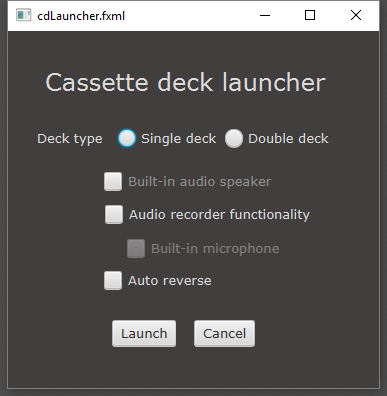
\includegraphics[width=7cm]{../img/launcher_final.png}\\
\end{center}
The cassette deck launcher allows the user to set the different functionalities the deck  has. In doing so, we are able to simulate distinct scenarios of different cassette deck models.\\
For example: if the user wishes so, they can check the "Audio recorder functionality" box, allowing them to also select the built-in microphone option, that being done, clicking on the "Launch" button will result in Recording features being enabled and ready to use.


\section{Single deck}
\vspace{10px}
\begin{center}
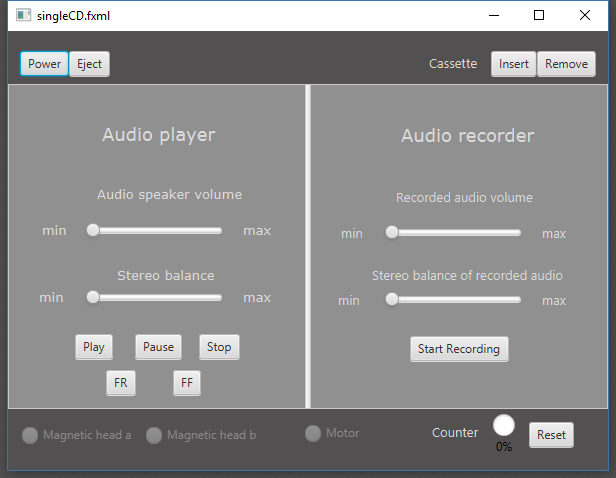
\includegraphics[width=15cm]{../img/singleDeck_final.png}\\
\end{center}
Depending on the features the user has chosen in the previous window (the launcher), some buttons and options might be disabled. For the sake of demonstration, we suppose that every features has been checked.\\
The user is greeted with a panel containing the main buttons, Power, Eject and Remove or Insert cassette, the last two are abstract in a real-world perspective (since these buttons do not exist in a cassette deck), but remain mandatory for executing the GUI.\\
Once a cassette is inserted, we are able to perform the two main functions of the deck, i.e. playing and recording audio, and all the related features.\\
The bottom panel contains disabled magnetic head radio buttons, showing which of the two is active in addition to a motor radio button, and one final button allowing the user to manually reset the counter.

\section{Double deck}
\vspace{10px}
\begin{center}
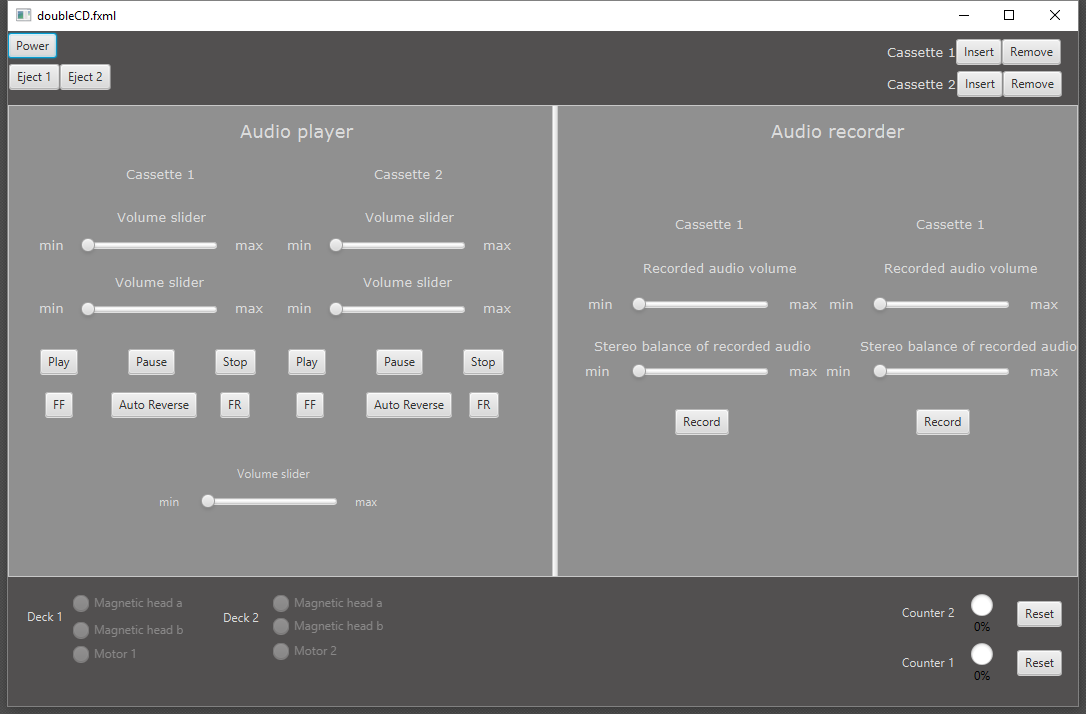
\includegraphics[width=16cm]{../img/doubleDeck_final.png}\\
\end{center}
Similar to the single deck, the double cassette deck provides not only the same, but additional features i.e. the option to play two cassettes simultaneously. The volume can be adjusted either by two separate volume sliders or a common one.\\
The Eject, Insert and Remove buttons are doubled, we also notice four magnetic heads, each two belonging to one deck. Motors and counters are also doubled.\\
It is possible to copy music from one cassette to the other by simply pressing play in the first deck and record on the second (or reversibly).
\pagebreak

\end{document}